




\begin{equation}\label{qn:dlb}
DLB(t, q_1, \cdots, q_n) = \dfrac { w_1(t) q_1 + \cdots + w_n(t) q_n } { \| w_1(t) q_1 + \cdots + w_n(t) q_n \| } 
\end{equation}
where
\begin{equation}
w_j(t) = \prod \limits _{\substack{k = 1 \\ k \neq j}} ^{n} \dfrac { t - t_k } { t_j - t_k }
\end{equation}






	
	\begin{tikzpicture}[scale=1, auto, >=stealth']
	\small
	% node placement with matrix library: 5x4 array
	\matrix[ampersand replacement=\&, row sep=0.2cm, column sep=0.4cm] {
		%
		\node[block] (F1) {$\vec{u}_i = F_i(\{\widetilde{\vec{x}}_j\}_{j=1}^N)$}; \&
		\node[branch] (u1) {}; \&
		\&
		\node[block] (f1) {$\begin{matrix}
			\dot{\vec{x}}_i =
			f_i(\vec{x}_i,
			\textcolor{red}{\{\widetilde{\vec{x}}_j\}_{j \myneq i}},
			\vec{u}_i,
			t)\\
			\vec{y}_i =
			g_i(\vec{x}_i,
			\textcolor{blue}{\{\widetilde{\vec{x}}_j\}_{j \myneq i}},
			t)
			\end{matrix}$}; \& \\
		
		\&
		\&
		\&
		\node[block] (L1) {$\vec{e}_i(\vec{y}_i - \widetilde{\vec{y}}_i)$};\&
		\node [sum] (e1) {}; \\
		
		\&
		\&
		\node[sum] (v1) {}; \&
		\node[block] (o1) {$\begin{matrix}
			\dot{\widetilde{\vec{x}}}_i =
			\widetilde{f}_i(\widetilde{\vec{x}}_i,
			\textcolor{red}{\{\widetilde{\vec{x}}_j\}_{j \myneq i}},
			\vec{v}_i, t)\\
			\widetilde{\vec{y}}_i =
			g_i(\widetilde{\vec{x}}_i,
			\textcolor{blue}{\{\widetilde{\vec{x}}_j\}_{j \myneq i}},
			t)
			\end{matrix}$};
		\&
		\\
		\node[guide] (i1) {}; \& \& \& \& \\
	};
	
	% now link the nodes
	\draw [line] (F1) -- (u1);
	\draw [connector] (u1) -- node {$u_i$} (f1);
	\draw [connector] (f1) -| node[near end] {$\vec{y}_i$} (e1);
	\draw [connector] (e1) -- (L1);
	\draw [connector] (L1) -| (v1);
	\draw [connector] (v1) -- node {$\vec{v}_i$} (o1);
	\draw [connector] (u1) |- (v1);
	\draw [connector] (o1) -| node[pos=0.96] {$-$} node [near end, swap]
	{$\widetilde{\vec{y}}_i$} (e1);
	\draw [connector] (o1.south) -- ++(0,-.5cm) -| node [near start]
	{$\widetilde{\vec{x}}_i$} ($(F1.south) + (0.4cm, 0em)$);
	
	% draw the snake lines with offset (using the calc library)
	\draw [snakeline] ($(i1) - (0.4cm, -1cm)$) -- node
	{$\{\widetilde{\vec{x}}_j\}_{j \myneq i}$} ($(F1.south) - (0.4cm, 0em)$);
	
	\draw [snakeline, swap] ($(v1.east) - (1.0cm, 0.4cm)$) -- node
	{$\{\widetilde{\vec{x}}_j\}_{j \myneq i}$} ($(o1.west) - (0cm, 0.4cm)$);
	
	\draw [snakeline, swap] ($(u1.east) + (0.1cm, -0.4cm)$) -- node
	{$\{\widetilde{\vec{x}}_j\}_{j \myneq i}$} ($(f1.west) - (0cm, 0.4cm)$);
	
	\end{tikzpicture}










% We need layers to draw the block diagram
\pgfdeclarelayer{background}
\pgfdeclarelayer{foreground}
\pgfsetlayers{background,main,foreground}

% Define a few styles and constants
\tikzstyle{sensor}=[draw, fill=blue!20, text width=5em, 
text centered, minimum height=2.5em]
\tikzstyle{ann} = [above, text width=5em]
\tikzstyle{naveqs} = [sensor, text width=6em, fill=red!20, 
minimum height=12em, rounded corners]
\def\blockdist{2.3}
\def\edgedist{2.5}

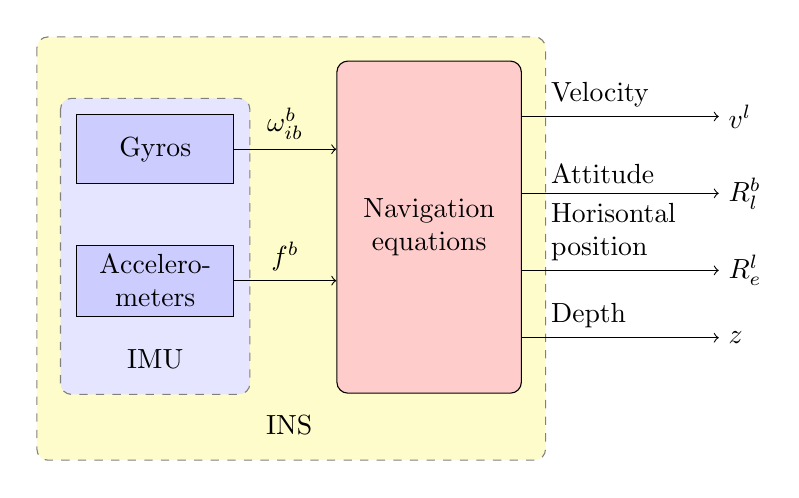
\begin{tikzpicture}
\node (naveq) [naveqs] {Navigation equations};
% Note the use of \path instead of \node at ... below. 
\path (naveq.140)+(-\blockdist,0) node (gyros) [sensor] {Gyros};
\path (naveq.-150)+(-\blockdist,0) node (accel) [sensor] {Accelero-meters};

% Unfortunately we cant use the convenient \path (fromnode) -- (tonode) 
% syntax here. This is because TikZ draws the path from the node centers
% and clip the path at the node boundaries. We want horizontal lines, but
% the sensor and naveq blocks aren't aligned horizontally. Instead we use
% the line intersection syntax |- to calculate the correct coordinate
\path [draw, ->] (gyros) -- node [above] {$\vc{\omega}_{ib}^b$} 
(naveq.west |- gyros) ;
% We could simply have written (gyros) .. (naveq.140). However, it's
% best to avoid hard coding coordinates
\path [draw, ->] (accel) -- node [above] {$\vc{f}^b$} 
(naveq.west |- accel);
\node (IMU) [below of=accel] {IMU};
\path (naveq.south west)+(-0.6,-0.4) node (INS) {INS};
\draw [->] (naveq.50) -- node [ann] {Velocity } + (\edgedist,0) 
node[right] {$\vc{v}^l$};
\draw [->] (naveq.20) -- node [ann] {Attitude} + (\edgedist,0) 
node[right] { $\mx{R}_l^b$};
\draw [->] (naveq.-25) -- node [ann] {Horisontal position} + (\edgedist,0)
node [right] {$\mx{R}_e^l$};
\draw [->] (naveq.-50) -- node [ann] {Depth} + (\edgedist,0) 
node[right] {$z$};

% Now it's time to draw the colored IMU and INS rectangles.
% To draw them behind the blocks we use pgf layers. This way we  
% can use the above block coordinates to place the backgrounds   
\begin{pgfonlayer}{background}
% Compute a few helper coordinates
\path (gyros.west |- naveq.north)+(-0.5,0.3) node (a) {};
\path (INS.south -| naveq.east)+(+0.3,-0.2) node (b) {};
\path[fill=yellow!20,rounded corners, draw=black!50, dashed]
(a) rectangle (b);
\path (gyros.north west)+(-0.2,0.2) node (a) {};
\path (IMU.south -| gyros.east)+(+0.2,-0.2) node (b) {};
\path[fill=blue!10,rounded corners, draw=black!50, dashed]
(a) rectangle (b);
\end{pgfonlayer}
\end{tikzpicture}










% The block diagram code is probably more verbose than necessary
\begin{tikzpicture}[auto, node distance=2cm,>=latex']
% We start by placing the blocks
\node [input, name=input] {};
\node [sum, right of=input] (sum) {};
\node [block, right of=sum] (controller) {Controller};
\node [block, right of=controller, pin={[pinstyle]above:Disturbances},
node distance=3cm] (system) {System};
% We draw an edge between the controller and system block to 
% calculate the coordinate u. We need it to place the measurement block. 
\draw [->] (controller) -- node[name=u] {$u$} (system);
\node [output, right of=system] (output) {};
\node [block, below of=u] (measurements) {Measurements};

% Once the nodes are placed, connecting them is easy. 
\draw [draw,->] (input) -- node {$r$} (sum);
\draw [->] (sum) -- node {$e$} (controller);
\draw [->] (system) -- node [name=y] {$y$}(output);
\draw [->] (y) |- (measurements);
\draw [->] (measurements) -| node[pos=0.99] {$-$} 
node [near end] {$y_m$} (sum);
\end{tikzpicture}










\tikzset{%
	block/.style    = {draw, thick, rectangle, minimum height = 3em,
		minimum width = 3em},
	sum/.style      = {draw, circle, node distance = 2cm}, % Adder
	input/.style    = {coordinate}, % Input
	output/.style   = {coordinate} % Output
}
% Defining string as labels of certain blocks.
\newcommand{\suma}{\Large$+$}
\newcommand{\inte}{$\displaystyle \int$}
\newcommand{\derv}{\huge$\frac{d}{dt}$}

\begin{tikzpicture}[auto, thick, node distance=2cm, >=triangle 45]
\draw
% Drawing the blocks of first filter :
node at (0,0)[right=-3mm]{\Large \textopenbullet}
node [input, name=input1] {} 
node [sum, right of=input1] (suma1) {\suma}
node [block, right of=suma1] (inte1) {\inte}
node at (6.8,0)[block] (Q1) {\Large $Q_1$}
node [block, below of=inte1] (ret1) {\Large$T_1$};
% Joining blocks. 
% Commands \draw with options like [->] must be written individually
\draw[->](input1) -- node {$X(Z)$}(suma1);
\draw[->](suma1) -- node {} (inte1);
\draw[->](inte1) -- node {} (Q1);
\draw[->](ret1) -| node[near end]{} (suma1);
% Adder
\draw
node at (5.4,-4) [sum, name=suma2] {\suma}
% Second stage of filter 
node at  (1,-6) [sum, name=suma3] {\suma}
node [block, right of=suma3] (inte2) {\inte}
node [sum, right of=inte2] (suma4) {\suma}
node [block, right of=suma4] (inte3) {\inte}
node [block, right of=inte3] (Q2) {\Large$Q_2$}
node at (9,-8) [block, name=ret2] {\Large$T_2$}
;
% Joining the blocks of second filter
\draw[->] (suma3) -- node {} (inte2);
\draw[->] (inte2) -- node {} (suma4);
\draw[->] (suma4) -- node {} (inte3);
\draw[->] (inte3) -- node {} (Q2);
\draw[->] (ret2) -| (suma3);
\draw[->] (ret2) -| (suma4);
% Third stage of filter:
% Defining nodes:
\draw
node at (11.5, 0) [sum, name=suma5]{\suma}
node [output, right of=suma5]{}
node [block, below of=suma5] (deriv1){\derv}
node [output, right of=suma5] (sal2){}
;
% Joining the blocks:
\draw[->] (suma2) -| node {}(suma3);
\draw[->] (Q1) -- (8,0) |- node {}(ret1);
\draw[->] (8,0) |- (suma2);
\draw[->] (5.4,0) -- (suma2);
\draw[->] (Q1) -- node {}(suma5);
\draw[->] (deriv1) -- node {}(suma5);
\draw[->] (Q2) -| node {}(deriv1);
\draw[<->] (ret2) -| node {}(deriv1);
\draw[->] (suma5) -- node {$Y(Z)$}(sal2);
% Drawing nodes with \textbullet
\draw
node at (8,0) {\textbullet} 
node at (8,-2){\textbullet}
node at (5.4,0){\textbullet}
node at (5,-8){\textbullet}
node at (11.5,-6){\textbullet}
;
% Boxing and labelling noise shapers
\draw [color=gray,thick](-0.5,-3) rectangle (9,1);
\node at (-0.5,1) [above=5mm, right=0mm] {\textsc{first-order noise shaper}};
\draw [color=gray,thick](-0.5,-9) rectangle (12.5,-5);
\node at (-0.5,-9) [below=5mm, right=0mm] {\textsc{second-order noise shaper}};
\end{tikzpicture}










\tikzstyle{block} = [draw, rectangle, 
minimum height=3em, minimum width=6em]
\tikzstyle{sum} = [draw, circle, node distance=1cm]
\tikzstyle{input} = [coordinate]
\tikzstyle{output} = [coordinate]
\tikzstyle{pinstyle} = [pin edge={to-,thin,black}]

% The block diagram code is probably more verbose than necessary
\begin{tikzpicture}[auto, node distance=2cm,>=latex']
% We start by placing the blocks
\node [input, name=input] {};
\node [sum, right of=input] (sum) {};
\node [block, right of=sum] (controller) {$G_c(s)$};
\node [block, right of=controller,
node distance=3cm] (system) {$G_p(s)$};
% We draw an edge between the controller and system block to 
% calculate the coordinate u. We need it to place the measurement block. 
\draw [->] (controller) -- node[name=u] {$U$} (system);
\node [sum, right of=system, node distance=2cm] (disturbance) {};
\node [block, above of=disturbance] (g_d) {$G_d(s)$};
\node [input, left of=g_d] (dist_input){$D$};
\node [output, right of=disturbance] (output) {};
\node [block, below of=u] (measurements) {$G_m(s)$};

% Once the nodes are placed, connecting them is easy. 
\draw [draw,->] (input) -- node {$Y_{sp}$} (sum);
\draw [->] (sum) -- node {$E$} (controller);
\draw [->] (system) -- node {$Y_u$} (disturbance);
\draw [->] (disturbance) -- node [name=y] {$Y$}(output);
\draw [->] (g_d) -- node {$Y_d$} (disturbance);
\draw [draw, ->] (dist_input) -- node {$D$} (g_d);
\draw [->] (y) |- (measurements);
\draw [->] (measurements) -| node[pos=0.99] {$-$} 
node [near end] {$Y_m$} (sum);
\end{tikzpicture}


In the context of the variables
\texttt{\{"query": "mycelium", "number": 100\}}, this would be expanded to
the very long  long URI \texttt{http://www.example.com/foo?query=mycelium\&number=100}. In the context of the variables
\mytexttt{\{"query": "mycelium", "number": 100\}}, this would be expanded to
the very long  long URI \mytexttt{http://www.example.com/foo?query=mycelium\&number=100}. In the context of the variables
\textvtt{\{"query": "mycelium", "number": 100\}}, this would be expanded to
the very long  long URI \textvtt{http://www.example.com/foo?query=mycelium\&number=100}.






